\documentclass[12pt]{article}
\usepackage{graphicx,import}
\usepackage[svgnames]{xcolor} 
\usepackage{fancyhdr}
\usepackage{subfig}
\usepackage{hyperref}
\usepackage{enumitem}
\usepackage{cite}
\usepackage[many]{tcolorbox}
\usepackage{listings }
\usepackage[a4paper, total={6in, 8in} , bottom = 25mm , top = 25mm, headheight = 1.25cm , includehead,includefoot,heightrounded ]{geometry}
\usepackage{afterpage}
\usepackage{amssymb}
\usepackage{fancyvrb}
\usepackage{pdflscape}
\usepackage{gensymb}
\usepackage{textcomp}
\usepackage{xecolor}
\usepackage{rotating}
\usepackage{pdfpages}
\usepackage[Kashida]{xepersian}
\usepackage[T1]{fontenc}
\usepackage{tikz}
\usepackage[utf8]{inputenc}
\usepackage{PTSerif} 
\usepackage{seqsplit}

\usepackage[edges]{forest}

\usepackage{listings}
\usepackage{xcolor}

\hypersetup{
	colorlinks   = true, %Colours links instead of ugly boxes
	urlcolor     = blue, %Colour for external hyperlinks
	linkcolor    = blue, %Colour of internal links
	citecolor   = red %Colour of citations
}
 
\definecolor{codegreen}{rgb}{0,0.6,0}
\definecolor{codegray}{rgb}{0.5,0.5,0.5}
\definecolor{codepurple}{rgb}{0.58,0,0.82}
\definecolor{backcolour}{rgb}{0.95,0.95,0.92}
 
\NewDocumentCommand{\codeword}{v}{
\texttt{\textcolor{blue}{#1}}
}
\lstset{language=java,keywordstyle={\bfseries \color{blue}}}

\lstdefinestyle{mystyle}{
    backgroundcolor=\color{backcolour},   
    commentstyle=\color{codegreen},
    keywordstyle=\color{magenta},
    numberstyle=\tiny\color{codegray},
    stringstyle=\color{codepurple},
    basicstyle=\ttfamily\normalsize,
    breakatwhitespace=false,         
    breaklines=true,                 
    captionpos=b,                    
    keepspaces=true,                 
    numbers=left,                    
    numbersep=5pt,                  
    showspaces=false,                
    showstringspaces=false,
    showtabs=false,                  
    tabsize=2
}

\lstset{style=mystyle}

\settextfont[Scale=1.2 ,BoldFont={Bahij Nazanin-Bold.ttf} , ItalicFont = {IRNazaninIranic.ttf}]{Bahij Nazanin-Regular.ttf}
\setlatintextfont[Scale = 1.0]{Garamond}
\DefaultMathsDigits 
\DeclareMathSizes{11}{19}{13}{9} 
%\DeclareMathSizes{12}{14.4}{8}{9}





\newenvironment{changemargin}[2]{%
\begin{list}{}{%
\setlength{\topsep}{0pt}%
\setlength{\leftmargin}{#1}%
\setlength{\rightmargin}{#2}%
\setlength{\listparindent}{\parindent}%
\setlength{\itemindent}{\parindent}%
\setlength{\parsep}{\parskip}%
}%
\item[]}{\end{list}}


\definecolor{foldercolor}{RGB}{124,166,198}

\tikzset{pics/folder/.style={code={%
    \node[inner sep=0pt, minimum size=#1](-foldericon){};
    \node[folder style, inner sep=0pt, minimum width=0.3*#1, minimum height=0.6*#1, above right, xshift=0.05*#1] at (-foldericon.west){};
    \node[folder style, inner sep=0pt, minimum size=#1] at (-foldericon.center){};}
    },
    pics/folder/.default={20pt},
    folder style/.style={draw=foldercolor!80!black,top color=foldercolor!40,bottom color=foldercolor}
}

\forestset{is file/.style={edge path'/.expanded={%
        ([xshift=\forestregister{folder indent}]!u.parent anchor) |- (.child anchor)},
        inner sep=1pt},
    this folder size/.style={edge path'/.expanded={%
        ([xshift=\forestregister{folder indent}]!u.parent anchor) |- (.child anchor) pic[solid]{folder=#1}}, inner xsep=0.6*#1},
    folder tree indent/.style={before computing xy={l=#1}},
    folder icons/.style={folder, this folder size=#1, folder tree indent=3*#1},
    folder icons/.default={12pt},
}

\begin{document}


%%% title pages
\begin{titlepage}
\begin{center}
        
\vspace*{0.7cm}


\includegraphics[width=0.4\textwidth]{sharif1.png}\\
\vspace{0.5cm}
\textbf{ \Huge{\emph ‌اندازه‌گیری و کنترل کامپیوتری} }\\
\vspace{0.5cm}
\textbf{ \Large{ تمرین پنجم} }
\vspace{0.2cm}
       
 
      \large \textbf{دانشکده مهندسی کامپیوتر}\\\vspace{0.2cm}
    \large   دانشگاه صنعتی شریف\\\vspace{0.2cm}
       \large   ﻧﯿﻢ سال دوم 00-99 \\\vspace{0.2cm}
      \noindent\rule[1ex]{\linewidth}{1pt}
استاد:\\
    \textbf{{جناب آقای دکتر همت‌یار}}


    \vspace{0.15cm}
نام و نام خانوادگی:\\

       
    \textbf{{امیرمهدی نامجو - 97107212}}
\end{center}
\end{titlepage}
%%% title pages


%%% header of pages
\newpage
\pagestyle{fancy}
\fancyhf{}
\fancyfoot{}
\cfoot{\thepage}
\chead{تمرین پنجم}
\rhead{
\includegraphics[width=0.1\textwidth]{sharif.png}}
\lhead{امیرمهدی نامجو}
%%% header of pages

\KashidaOff


\section*{سوال 3}

فاصله اولیه $1mm$ است. در فاصله $1.02mm$ داریم:
$$C = 880 \times 1/1.02 = 862.7 pF$$
در فاصله $0.98mm$ داریم:
$$C = 880 \times 1/0.98 = 898.0 pf$$

بازه تغییرات حدودا $\pm 18pF$ است. اختلاف دو بازه $36 pF$ است.

\section*{سوال 6}


\begin{enumerate}
	\item 
	
	
	$$2.5 \times 10^{-3} \times 200 = 0.5V$$
	
	پس بازه تغییرات بین $-0.5V$ تا $0.5V$ است.

\item

$$(+ 200 - (-200)) / 0.5 =800$$

یعنی به $800$ حالت نیاز داریم. پس حداقل نیاز به $10$ بیت داریم.


\item

در واقع بازه بین $-0.5$ تا $0.5$ ولت را باید به بازه $-2.5$ تا $2.5$ ببریم و خروجی را به ADC بدهیم. در نتیجه Gain مدار $5$ است. با مدار غیرمعکوس کننده زیر می توان این کار را انجام داد.

\begin{center}
	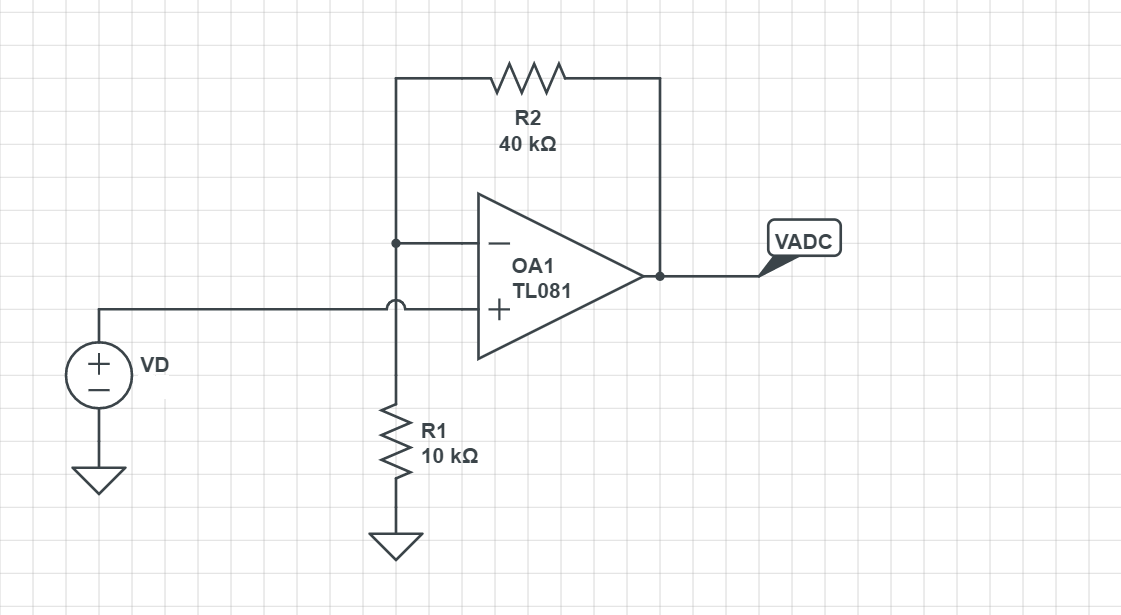
\includegraphics[width = 1.0 \textwidth]{images/1.png}
\end{center}	

البته در اصل اگر بخواهیم دقیق باشیم، بازه مد نظر ما بین $-2.5$ تا $2.5 -2.5/1024$ است. در این صورت با حل دو معادله دو مجهول به عبارت
$$V_{adc} = (4.99756) V_{D} - 0.0012 =(4.99756)(V_{D} - 0.00025) $$
می شد که به دلیل کوچک بودن عرض از مبدا، از در نظر گرفتن آن صرف نظر شده است.
\end{enumerate}

\newpage
\section*{سوال 9}

مداری مطابق شکل زیر طراحی می کنیم:

\begin{center}
	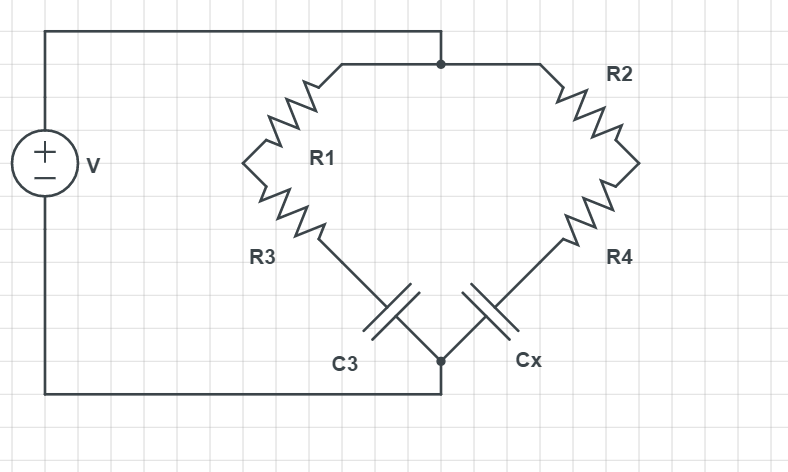
\includegraphics[width = 0.5 \textwidth]{images/2.png}
\end{center}

$$R_{1} (R_4 + 1/(j \omega C_x) ) = R_2 (R_3 + 1/(j \omega C_3))$$

در نتیجه:

$$R_1 R_4 = R_2 R_3$$
$$R_1/(\omega C_x) = R_2 / (\omega C_3)$$

با توجه به اعداد داده شده در صورت سوال و همچنین مثال 4 کتاب، نقطه Null را برابر $C_x = 0.0032 \mu F$ در نظر گرفته و داریم:

$$R_1 = R_3 = 1 k\Omega , C_3 = 0.02 \mu F , C_x = 0.0032 \mu F , \omega = 1 \times 2 \pi $$

و از حل معادله بدست می آید:
$$R_2 = 6250 \Omega $$

حال برای رسم نمودار باید مقاومت کل را برحسب سطح اتیل الکل بدست آوریم. در مثال 4 کتاب $A=1.806 m^2$ بدست آمده بود و کل طول ظرف هم $5m$ بود. در نتیجه اگر $x$ متر اتیل الکل باشد $5-x$ متر هوا است. خازن ها هم موازی بوده و مقادیرشان جمع می شود. پس

$$C_x = \epsilon_0 \times (1.806 / 0.005) \times (K_{ethyl} x + K_{air} \times 5 - K_{air} x) = 3197 (25x + 5) pF$$

از طرف دیگر برای اختلاف ولتاژ بین دو سر پل داریم:

$$\delta V = V (\frac{R_3 + 1/j \omega C_3}{R_3 + 1/j \omega C_3 + R_1} - \frac{R_4 + 1/j \omega C_x}{R_4 + 1/j \omega C_x  + R_2})$$

با جایگذاری این موارد و فاکتور گیری از توان های مشترک در صورت و مخرج داریم:

$$
\Delta V = 5 \left[\frac{1-7.96 j}{2-7.96 j}-\frac{6.25-j \frac{498}{25 x+5}}{12.5-j \frac{498}{25 x+5}}\right]
$$

با رسم نمودارها به کمک \lr{Wolfram Mathematica} داریم:

نمودار Magnitude برحسب V نسبت به Level برحسب متر:


\begin{center}
	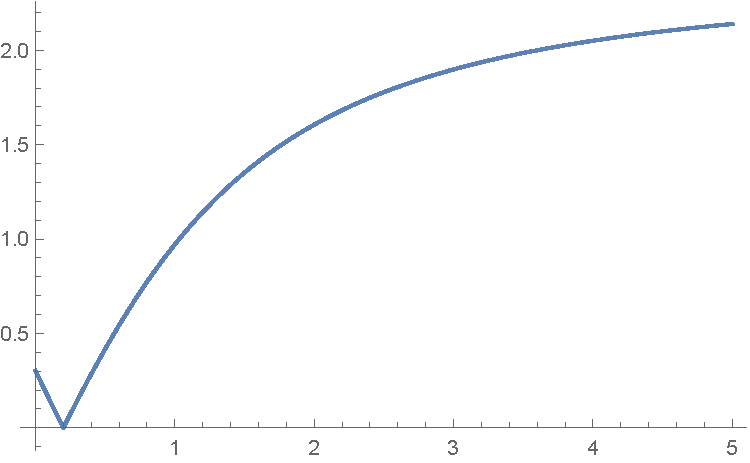
\includegraphics[width = 1.0 \textwidth]{images/3.pdf}
\end{center}

نمودار فاز برحسب درجه نسبت به Level برحسب متر:

\begin{center}
	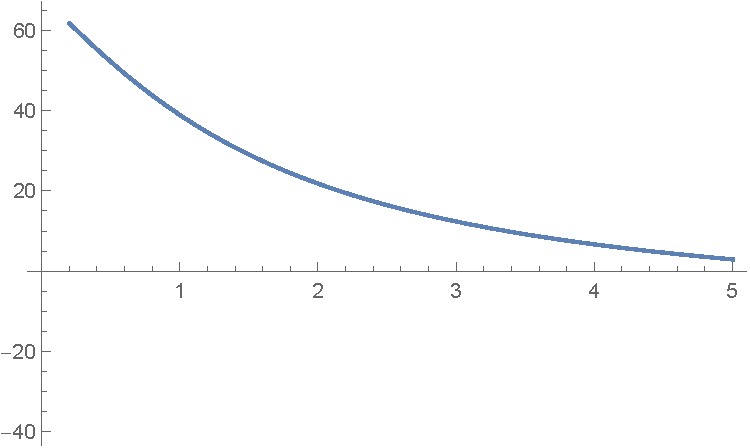
\includegraphics[width = 1.0 \textwidth]{images/4.pdf}
\end{center}

\newpage

\section*{سوال 12}

$$\Delta R = GF \times R \times (strain) = 2.06 \times 120 \times 10^{-6} = 2.472 \times 10^{-4}$$

از فرمول فصل قبل داریم:

$$\Delta R = \alpha_0 R \Delta T$$
$$\Delta T = (2.472 \times 10^{-4}) \times (0.0034) \times 120 = 1 \times 10^{-4} \deg C$$

از طرفی 
$\delta T = P/P_D$
و
$P=I^2 R$
پس
$$I = \sqrt{(P_D \Delta T / R)} = \sqrt{(25 \times 10^{-3} \times 1 \times 10^{-4} \times 120)} = 300 \mu A$$


\newpage

\section*{سوال 15}

داریم:

$$\Delta V = V_s (\frac{R_D}{R_1 + R_D} - \frac{R_A}{R_A + R_2})$$

و
$$R_A = R(1 + \frac{\Delta R}{ R})$$

در نتیجه:

$$\Delta V = V_s (\frac{R}{2R } - \frac{R(1 + \frac{\Delta R}{ R})}{R(1 + \frac{\Delta R}{ R}) + R}) = \frac{V_s}{2}(1 - \frac{(1 + \frac{\Delta R}{ R})}{(1 +\frac{1}{2} \frac{\Delta R}{ R})})$$

$$= \frac{V_s}{2} \frac{-\frac{1}{2} \frac{\Delta R}{R}}{1 + \frac{1}{2} \frac{\Delta R}{R}}$$

همچنین با توجه به بسط تیلور می دانیم:

$$\frac{1}{1+x} = 1 -x + x^2/2! - ...$$

در نتیجه:

$$\Delta V \approx \frac{V_s}{2} (-\frac{1}{2} \frac{\Delta R}{R}) (1 - \frac{1}{2} \frac{\Delta R}{R}) \approx -\frac{V_s}{4} \frac{\Delta R}{R}$$

و با توجه به فرمول GF داریم:

$$\Delta V = -\frac{V_s}{4} GF \frac{\Delta l}{l}$$

\newpage

\section*{سوال 18}

ماژول یانگ برای مس حدود 
$11.73 \times 10^{11} N/m$
است. داریم:

$$E=(F/A) / (strain)$$

$$\pi R^2 = \pi(6/2 \times 0.0254)^2 = 1.824*10^{-2} m^2$$

$$strain = (1 lb \times (4.448 N/lb)) / (1.842 \times 10^{-2} \times 11.73 \times 10^{11}) = 2.06 \times 10^{-10}$$

$$\Delta R = R \times (2.02) \times (2.06 \times 10^{-10}) = 4.99 \times 10^{-8} \approx 5 \times 10^{-8} \Omega$$

شکل تقریبی آن به این صورت خواهد بود  و با توجه به فشرده شدن، مقاومت کاهش خواهد یافت:

\begin{center}
	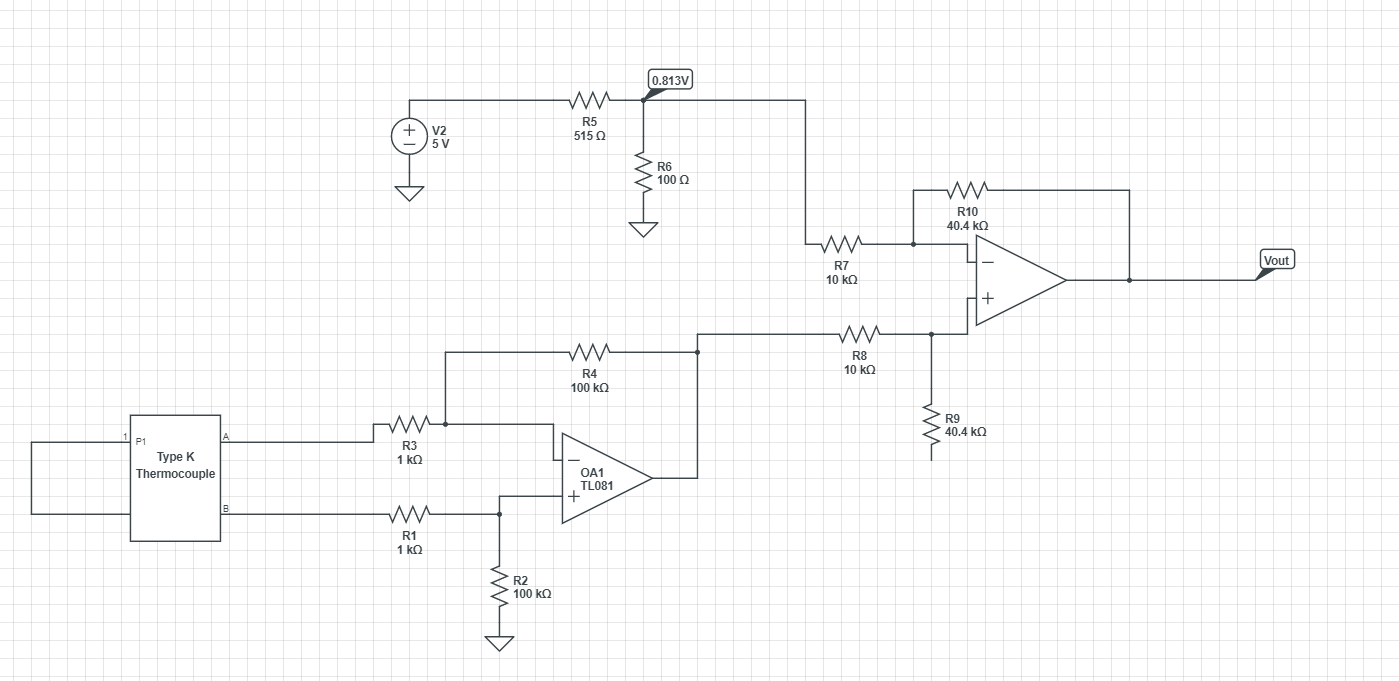
\includegraphics[width = 1.0 \textwidth]{images/6.png}
\end{center}


\newpage

\section*{سوال 21}

$$10000 \frac{round}{m} \times 2 \pi\frac{rad}{round} \times (1 m/ 60 s) = 1047.2 rad/s$$


\section*{سوال 24}

$$2 g \Delta X = v^2 \rightarrow v = \sqrt{2 \times 9.8 \times 1.5} = 5.42 m/s$$

$$a_2 = \Delta V / \Delta T = (5.42) / (2.7 \times 10^{-3}) \times (1/9.8) = 204.8 g$$

\section*{سوال 27}

\begin{enumerate}
	\item
	
	$$V = (0.31 mV/mm) \Delta X = 0.31 \Delta x$$
	
	از طرفی
	$$k \Delta x = m a \rightarrow \Delta x = \frac{m}{k}a$$
	
	پس
	$$V = (0.31) (m/k) a = 0.31 (0.05 /240) a = (6.46 \times 10^-5) a$$
	
	\item
	
	$$V_max = (0.31 V/m) \times (2 cm) = 0.31 \times 2 \times 10^{-2} = 6.2 mV $$
	
	$$a = 1/(6.46 \times 10^{-5}) \times (\pm 6.2 \times 10^{-3}) = \pm 95.97 \approx \pm 96 m/s^2$$
	
	\item
	
	$$f_n = \frac{\sqrt{\frac{k}{m}}}{2 \pi } = \frac{\sqrt{\frac{240}{0.05}}}{2 \pi } = 11.02 \approx 11 Hz$$
\end{enumerate}


\section*{سوال 30}

داریم:

$$E = \frac{F}{A} / \frac{\Delta l}{l}$$

$$\frac{\Delta R} { R} = GF (\frac{\Delta l}{l})$$
$$F=ma$$

$$\frac{\delta R}{R} = \frac{GF m a}{E A}$$

از آن جایی که به ازای واحد $g$ می خواهیم مقدار $a=9.8m/s^2$ گذاشته و بقیه را هم از صورت سوال جایگزین می کنیم:

$$\delta R = 120 \Omega \times (\frac{9.8 m/s^2 \times 2.03 \times0.02 kg }{10^8 N/m^2 \times 2 \times 10^{-4} m^2}) = 2.39 \times 10^{-3} \Omega$$

یعنی نرخ تغییر مقاومت به ازای هر $g$ برابر 
$2.39 \times 10^{-3} \frac{\Omega}{g}$
است.


\section*{سوال 33}

$$1500 psi / (1.45 \times 10^{-4} psi/Pa) = 10.3 \times 10^6 Pa$$

$$1500 psi / (14.7 psi /\text{atmosphere}) =  102.04 \text{atmosphere}$$

\end{document}



